\section{Parking Lot Generation}

Once the plot generation is finished the parking lot generation starts working towards filling some of the generated plots with parking lots.

The generated parking lots consist of one or more rows of parking spaces (see Figure~\ref{fig:results_parking_sizebased}).

\begin{figure}[H]
   \centering
   \begin{subfigure}[b]{0.485\textwidth}
     \frame{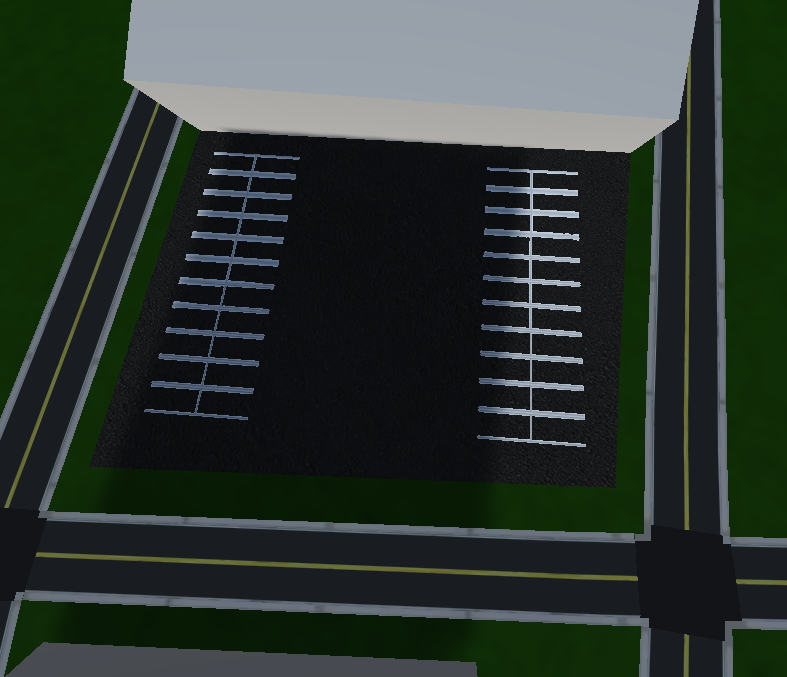
\includegraphics[width=\textwidth]{figure/results/parking/bigplot.png}}
     \caption{Large parking lot consisting of two rows.}
   \end{subfigure}
   \quad
   \begin{subfigure}[b]{0.45\textwidth}
     \frame{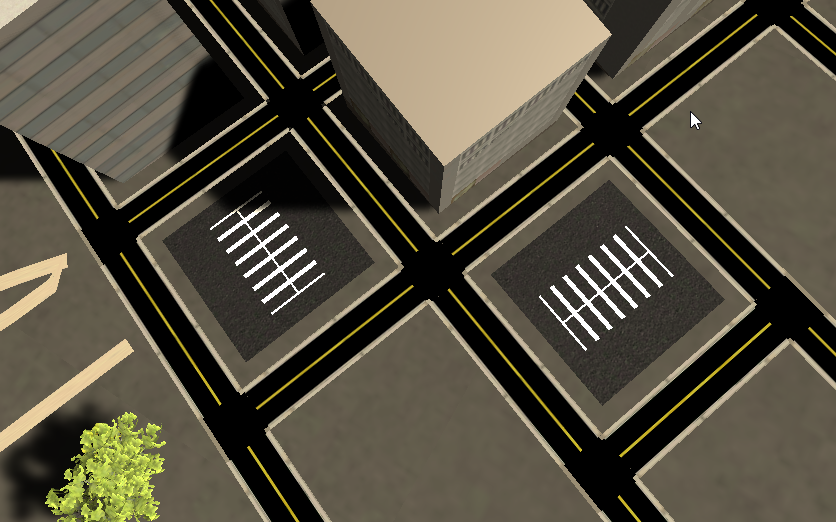
\includegraphics[width=\textwidth]{figure/results/parking/smallplots.png}}
     \caption{Two small parking lots consisting of one row.}
   \end{subfigure}
     \caption{Two examples of different sized parking lots created by the generator.}
   \label{fig:results_parking_sizebased}
 \end{figure}

These parking lots are generated by calculating the largest possible rectangle inside a polygon, and then generating parking lots inside them.
The number of rows is based on the size of the approximated rectangle, and the algorithm aims to fit as many rows of parking lots inside the rectangle such that there are still space between the rows for cars to enter.

Having the parking lots consist of multiple rows depending on the size gives some more variety, but the decision to do this was also based on real-world parking lots (see Figure~\ref{fig:parkings}).
From the left image it is obvious that not having a road separate the rows would make it possible for a car to be entirely parked and unable to move.
The right image however has a more interesting shape, the parking lot in the center of it is shaped in the two-row style, however the surrounding rectangle is large enough that cars can easily drive around and not be blocked by parked cars.
This type of parking space is difficult to generate reliably in arbitrary plot shapes, and as such was not implemented in the generator.

\begin{figure}[H]
  \centering
  \begin{subfigure}[b]{0.55\textwidth}
    \frame{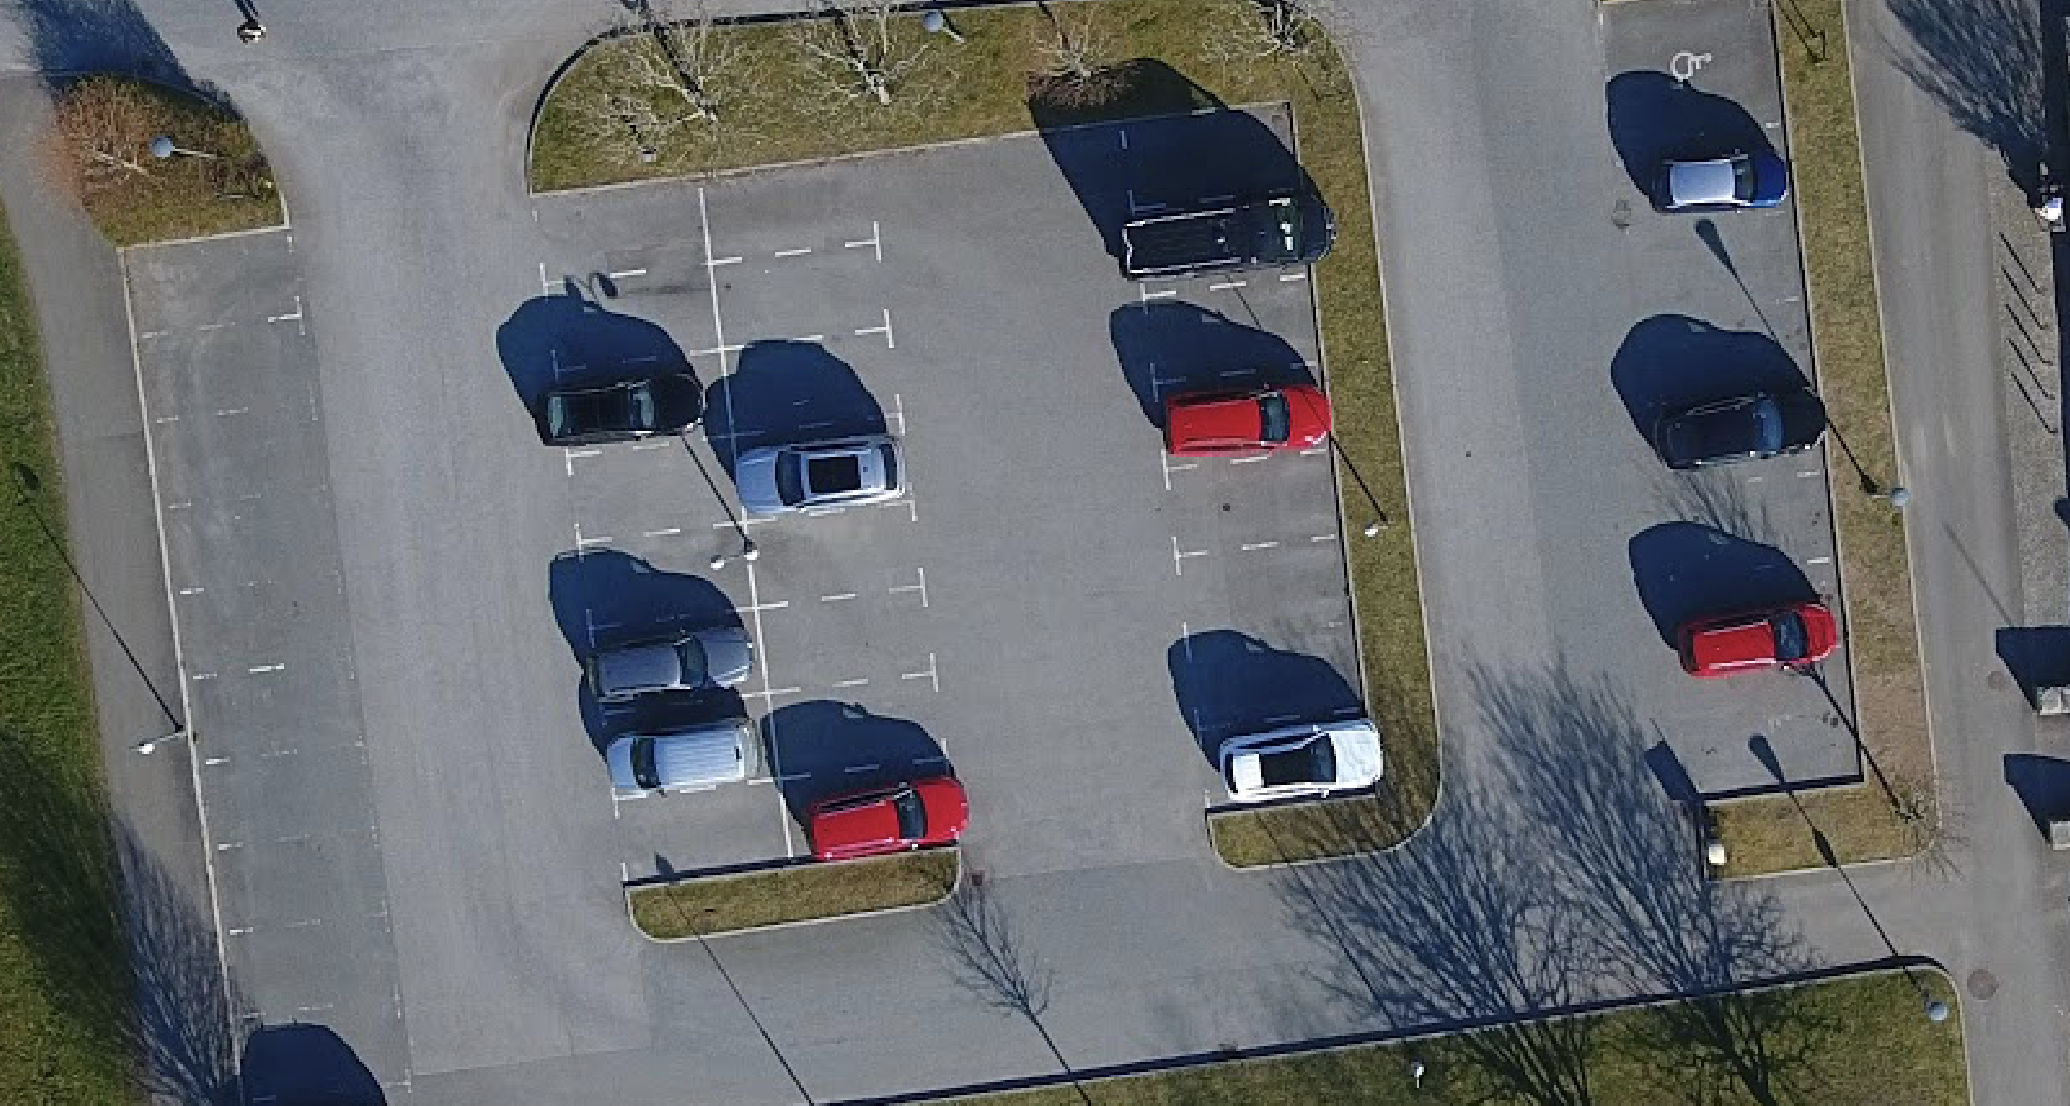
\includegraphics[width=\textwidth]{figure/results/parking/real1.png}}
  \end{subfigure}
  \quad
  \begin{subfigure}[b]{0.395\textwidth}
    \frame{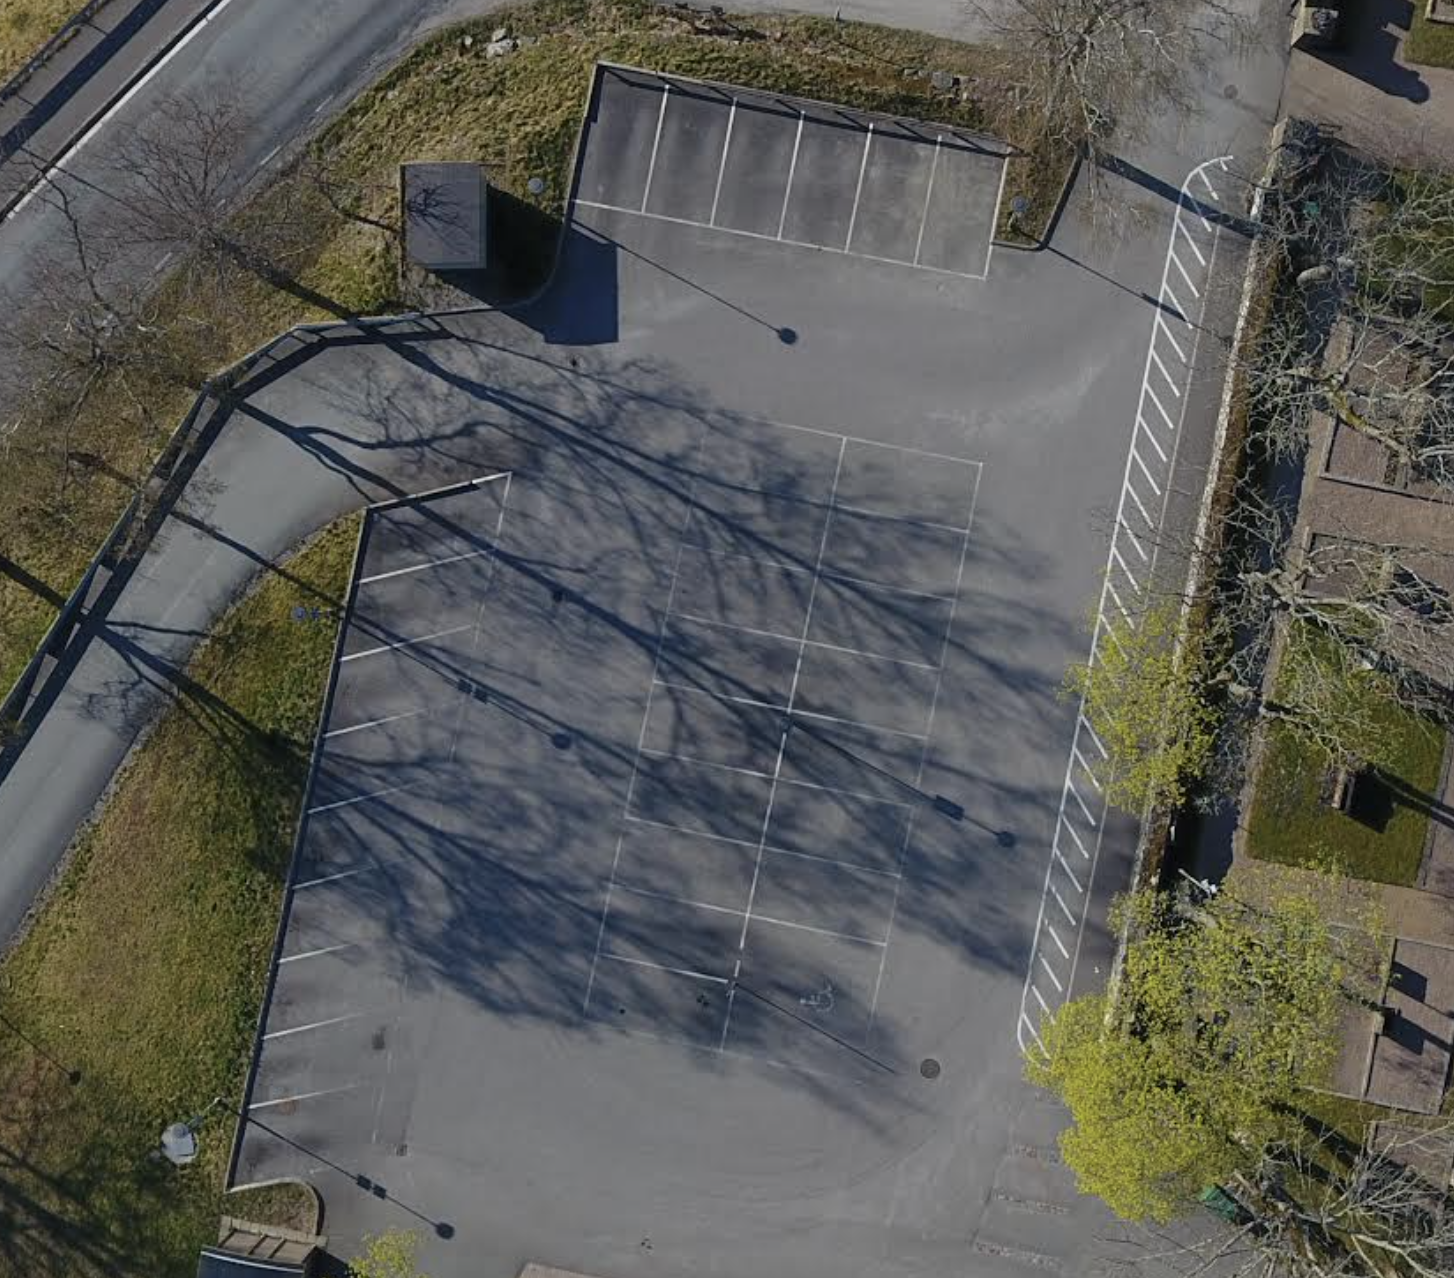
\includegraphics[width=\textwidth]{figure/results/parking/real2.png}}
  \end{subfigure}
  \caption{Two examples of parking lots observed by the project group, showcasing the rectangular shapes mentioned above.}
  \label{fig:parkings}
\end{figure}
